\documentclass{article}
\usepackage{graphicx}
\usepackage{tabularx}
\usepackage{fancyhdr}
\usepackage{cite}
\usepackage{hyperref}
\usepackage{lipsum}
\usepackage{xcolor}
\usepackage{colortbl}

\pagestyle{fancy}
\setlength{\footskip}{60pt}
\vspace{-2cm}
\fancyfoot{\rule{0.5\linewidth}{1pt}}

\fancyfoot[L]{{
\includegraphics[scale=0.10]{logo.png}}}

\definecolor{lightgreen}{rgb}{0.56, 0.93, 0.56}

\begin{document}


\begin{center}

\includegraphics[scale=0.2]{logo.png}
\end{center}

\vspace{0.5cm}

\begin{center}

 Team's name: FamilyName1, FamilyName2, FamilyName3, FamilyName4 \\

\vspace{0.5cm}

{\Huge \textcolor{red}{Recovery and stress meter}} \\


\vspace{0.5cm}

{\Large \textbf{Project plan}} \\


\end{center}

\vspace{1cm}

\begin{center}

{\Large }



\begin{tabular}{l}
 First year hardware project \\
 School of ICT\\
 Metropolia University of Applied Sciences  \\
 \today \, (v0.2)
\end{tabular}
\end{center}

\newpage

\begin{abstract}
Write your abstract here.
\end{abstract}




\begin{center}
\textbf{\large Keywords:}
\end{center}

\vspace{1cm}

\begin{table}[h]
\centering
\begin{tabular}{|p{1cm}|p{4cm}|c|c|}
\hline
\textbf{Ver} & \textbf{Description} & \textbf{Date} & \textbf{Author(s)} \\ \hline
0.1 & First version created from the Construx's software development plan template. & 9.12.2022 & Sakari Lukkarinen \\ \hline
0.2 & Continued editing. Added examples and other documents. & 11.12.2022 & Sakari Lukkarinen \\ \hline
 &  &  &  \\ \hline
 &  &  &  \\ \hline
 &  &  &  \\ \hline
 &  &  &  \\ \hline
\end{tabular}
\caption{Version history}
\label{table:version-history}
\end{table}

\begin{bf}
\begin{center}
\fbox{
\parbox{0.8\textwidth}{
Keyword 1\\ Keyword 2 \\ Keyword 3 \\
...
}
}
\end{center}
\end{bf}

\newpage

\tableofcontents

\section{Introduction}
This section describes the recovery and stress meter project being to be
conduct during the first year Hardware courses of School of ICT at Metropolia
University of Applied Sciences.



\subsection{Project Overview and Vision}
The objective of the project is to create a proof-of-concept product of a stress and
recovery meter. The project begins with the discovery phase, where the
requirement specification is reviewed, the project plan is developed with detailed
schedule and risk management plans. The planning checkpoint review is
arranged at the beginning of the 4th learning period starting in the middle of
March.

In the 4th learning period, the project continues to the invention phase where the
architecture of the system and detailed design are planned. The actual
implementation work is divided into three (3) iterative development stages each
of them having a separate release and milestones. The final release is at the end
of the spring semester.

During the development the project plan with time schedules and risk
management are updated under change and version control.


\subsection{Project Deliverables}
The main deliverables of the project are:
\begin{itemize}
\item The updated and detailed requirement specification
\item The project plan (this document)
\item Architecture and detailed design document (to be developed in the 4th period)
\item The proof-of-concept product (the product)
\item User's manual for the product
\item documented source codes.
\end{itemize}


The main deliverables, their release dates, physical locations and delivery
methods are listed in Table \ref{tab:deliverable}.

\begin{table}[h]
\centering
\caption{The main deliverables of the project.}
\label{tab:deliverable}
\begin{tabular}{|l|l|l|l|}
\hline
\textbf{Main deliverable} & \textbf{Release date} & \textbf{Physical location} & \textbf{Delivery method} \\
\hline
Detailed requirement specification & TBD & TBD & TBD \\
\hline
Project plan & TBD & TBD & TBD \\
\hline
Architecture design & TBD & TBD & TBD \\
\hline
Detailed design & TBD & TBD & TBD \\
\hline
User’s manual & TBD & TBD & TBD \\
\hline
Source code and its documentation & TBD & TBD & TBD \\
\hline
Proof-of-concept product & TBD & TBD & TBD \\
\hline
\end{tabular}
\end{table}


\subsection{Evolution of the Project Management Plan}
The following Table \ref{tab:deliverable} summarises the project management plan showing the
version, primary authors, description and data completed estimates.

\begin{table}[h]
\centering
\caption{Project management plan.}
\label{tab:project_management_plan}
\begin{tabular}{|l|p{2cm}|p{7cm}|p{2cm}|}
\hline
\textbf{Version} & \textbf{Primary author(s)} & \textbf{Description} & \textbf{Date completed} \\
\hline
Draft & & Initial draft created for distribution and review comments & TBD \\
\hline
Preliminary & & Second draft incorporating initial review comments distributed for final review & TBD \\
\hline
Final & & First complete draft, which is placed under change control & TBD \\
\hline
Revision 1 & & Revised draft, revised according to the change control process and maintained under change control & TBD \\
\hline
Revision 2 & & Second revision, revised according to the change control process and maintained under change control & TBD \\
\hline
Revision 3 & & Third revision, revised according to the change control process and maintained under change control & TBD \\
\hline
\end{tabular}
\end{table}

\subsection{Reference Materials}
Below is listed all the documents and other materials referenced in this document.

Documents
\begin{itemize}
\item Requirements Specifications (v0.7), 11.12.2022, Author(s): Sakari Lukkarinen, Word document.
\item Requirements Specifications, Functional and non-functional requirements, user roles and use cases (v0.7), 11.12.2022, Author(s): Sakari Lukkarinen, Excel document.
\item Gantt timetable (v0.2), 11.12.2022, Author(s): Sakari Lukkarinen, Excel document.
\item Risk evaluation and management, Last update 11.12.2022, Author(s): Sakari Lukkarinen, Excel document.
\end{itemize}


Other materials
\begin{itemize}
\item McConnell, S. (1998). Software Project Survival Guide. MicroSoft Press.
\item Harrin, E. (2017). How to Create a Project Organization Chart. ProjectManagement.com
\item Wikipedia, Product-based planning in Project management. Accessed 11.12.2022.
\item Wikipedia, PRINCE2. Projects in controlled environments a structured project management method. Accessed 11.12.2022.
\item Wrike, What Is a Work Package in Project Management? wrike.com. Accessed 11.12.2022.
\end{itemize}

\subsection{Definitions and Acronyms}

TBD.

\textcolor{red}{Instructions: Provide definitions or references to all the definitions of the special terms and acronyms used within this document.}

\textcolor{red}{This could probably be also done on the beginning of the article.}

\section{Project Organization}
A staged delivery plan is followed having at least 3 stages and the final release.
The project’s process model, organizational structure (chain of command and
management reporting structure), and responsibilities of individuals on the project
are described in this chapter.



\subsection{Process Model}
A staged delivery plan is followed in the project. A detailed GANTT chart of major
phases and milestones are given in a separate document \textcolor{red}{(XXX. Project Phases
and Milestones)}. The following Table \ref{tab:work_product_status} summarises the major work products,
their planned completion dates and their content.

[table]
\begin{table}[h]
\centering
\caption{ Major work products and their content and timing.}
\label{tab:work_product_status}
\begin{tabular}{|p{2cm}|p{2cm}|p{2cm}|p{2cm}|p{2.2cm}|}
\hline
\textbf{Work product name} & \textbf{Planned completion date} & \textbf{Placed under change control} & \textbf{Deliverable to customer} & \textbf{Approved by} \\
\hline
TBD & TBD & Yes & No & Project manager  \\
\hline
 TBD & TBD & No & Yes & Engineering lead  \\
\hline
 TBD & TBD & Yes & Yes & Documentation  \\
\hline
\end{tabular}
\end{table}

\textcolor{red}{Instructions: consider including all the top-level work products.}

\subsection{Organizational Structure and Project Responsibilities}
Each major project responsibility and the responsible persons are described in
Table \ref{tab:project_responsibilities}.

\begin{table}[h]
\centering
\caption{Project responsibilities and persons responsible.}
\label{tab:project_responsibilities}
\begin{tabular}{|l|l|}
\hline
\textbf{Responsibility} & \textbf{Persons responsible} \\
\hline
Overall Project Manager & TBD \\
\hline
Engineering Manager & TBD \\
\hline
Quality Assurance Manager & TBD \\
\hline
End-User Documentation Manager & TBD \\
\hline
Requirements Development & TBD \\
\hline
Software Architecture & TBD \\
\hline
Technical Self-Review & TBD \\
\hline
Etc. & TBD \\
\hline
\end{tabular}
\end{table}



The project’s internal structure, the lines of authority, responsibility and
communication within the project are illustrated in Figure \ref{harrin} .


\begin{figure*}[h]
  \centering
  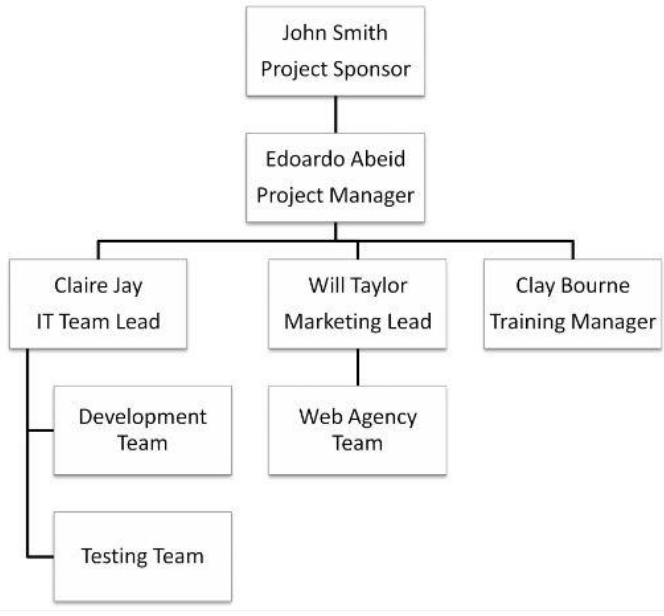
\includegraphics[width=0.7\textwidth]{harrin_2017.png}
  \caption{ Example of project's organisational chart (Source: Harrin, 2017).}
  \label{harrin}
\end{figure*}




\section{Managerial Process}
The management objectives, priorities, project assumptions, dependencies, constraints, risk management techniques, monitoring and controlling mechanisms, and the staffing plan are described here.




\subsection{Management Objectives and Priorities}
The project is managed following the product-based planning and PRINCE2
structured project management method (See other documents for details).
\textcolor{red}{Instructions: Describe the philosophy, goals, and priorities for management
during the project. Consider including the following items:}

\begin{itemize}
\item {\color{red}status reporting}
\item {\color{red}relative priorities among functionality, schedule, and budget}
\item {\color{red}risk management procedures}
\item {\color{red}approach to modifying existing software}
\end{itemize}

\subsection{Assumptions, Dependencies, and Constraints}
The project plan is based on the given preliminary requirement specification and
documents (See 1.4 Reference Materials).
The project’s schedule is constrained to the Spring 20\textcolor{red}{XX} semester, which ends
at \textcolor{red}{XX.XX.20XX}. Totally \textcolor{red}{XX} engineering students are involved on the project
development process.
The project’s time budget is based on the ECTS system. Each ECTS point is
budgeted for 27 hours of study work. Totally \textcolor{red}{XXX} hours of engineering students’
workhours are used for the project.
The quality measures of the project are being updated during the project. The
quality of the final proof-of-concept is constrained by the given schedule, time
budget, and human resources. Based on these constraints, the proof-of-concept
product is planned to have the functionalities given in the detailed requirement
specification (See Document \textcolor{red}{XXX}). However, any guarantees of the quality of the
implemented features cannot be given, but the results are as-they-are.
\subsection{Risk Management}

A separate risk evaluation and management document is given in document \textcolor{red}{XXX}.
The Table \ref{tab:project_risks} lists the top major risks for the project.

\begin{table}[h]


\centering
\caption{Major identified and evaluated risks of the project. \textcolor{red} {Instructions: copy
here the initial top 10 risk list and update the table at major milestones of the
project. }}

\label{tab:project_risks}
\begin{tabular}{|c|l|c|c|c|}
\hline
\textbf{ID} & \textbf{Description} & \textbf{Severity} & \textbf{Likelihood} & \textbf{Risk level} \\
\hline
R\_01 & Unachieavable schedule & 3 & 3 & \cellcolor{yellow} 9 \\
\hline
R\_02 & Released product has low quality & 2 & 4 & \cellcolor{yellow} 8 \\
\hline
R\_03 & Requirements or developer gold plating & 2 & 2 & \cellcolor{lightgreen} 4 \\
\hline
R\_04 & Creeping requirements & 1 & 3 & \cellcolor{lightgreen} 3 \\
\hline
R\_05 & Unstable tools delay schedule & 1 & 1 & \cellcolor{green} 1 \\
\hline
R\_06 & TEST very high risk & 4 & 4 & \cellcolor{red} 16 \\
\hline
R\_07 & TEST very low risk & 1 & 1 & \cellcolor{green}  1 \\
\hline
R\_08 & TEST another very high risk & 4 & 4 & \cellcolor{red} 16 \\
\hline
\end{tabular}
\end{table}

\subsection{Monitoring and Controlling Mechanisms}
The project shedule, quality and functionality are tracked through the project. The
report content and format follows .... \textcolor{red}{Instructions: describe here the report content and format}.

\vspace{0.5cm}

The monitoring report is structured the following way ... \textcolor{red}{ Instructions: write here
the report structure} and they are delivered every  \textcolor{red}{XXX} week.

\vspace{0.5cm}

The project progress is controlled ... \textcolor{red}{Instructions: write here how the project progress is controlled}.

\subsection{Staffing Plan}

\textcolor{red}{Instructions: Describe the numbers and types of personnel needed to conduct the
project, for example: NN engineering students with ... skill levels are required.
The project starts at ...... and continues XXX weeks. The personnel are selected
by (method of obtaining the personnel), and (what?) training is required. All staff
is phased out at the end of the project.}

\section{Technical Process}
The top-level technical processes used on the project including the technical
methods, tools, and techniques; major software documents; and supporting
activities such as configuration management and quality assurance are described
in this chapter.

\subsection{Methods, Tools and Techniques}
The following methods, tools and techniques are used in the project {\color{red} (see the
requirement specification for more details):


\begin{itemize}
\item The computing system environment including hardware and operating system environment: ....
\item Software tools including design tools, source code control, time accounting, compiler or IDE, debugging aids, defect tracking, and so on: ...
\item Development methodologies including requirements development practices, design methodologies and notations, programming language, coding standards, documentation standards, system integration procedure, and so on (these will not all be defined when the first draft of the project plan is created; the section should be updated as the plans become more detailed)
\item Quality assurance practices including methods of technical peer review, unit testing, stepping through code in a debugger, system testing, automated regression tests, and so on: ....
\end{itemize}
}

\subsection{Documentation}
The following documents will be developed for the project:

\textcolor{red}{Instructions: List here all the major documents ...}

\subsection{Project Support Functions (optional)}
\textcolor{red}{
Instructions: Describe here or give references to other documents that describe
the plans for functions that support the software development effort, including
configuration management, quality assurance, and end user documentation.
Describe the responsibilities, resource requirements, schedule, budget, and so
on. Note: this section can be added later during the project.}

\section{Work Packages, Schedule, and Budget}
\subsection{Work Packages and their dependencies}
\textcolor{red}{Instructions: Create a first draft of work packages and place them here (i.e., task
or collection of tasks that must be completed to complete the product).
Identify each work package with a unique number and provide a diagram showing
the breakdown of work packages into sub-packages (See Figure \ref{wrike} for example).
Describe the dependencies both among work packages, and external events.
Update this part in every stage when the project progresses.}

\begin{figure*}[h]
  \centering
  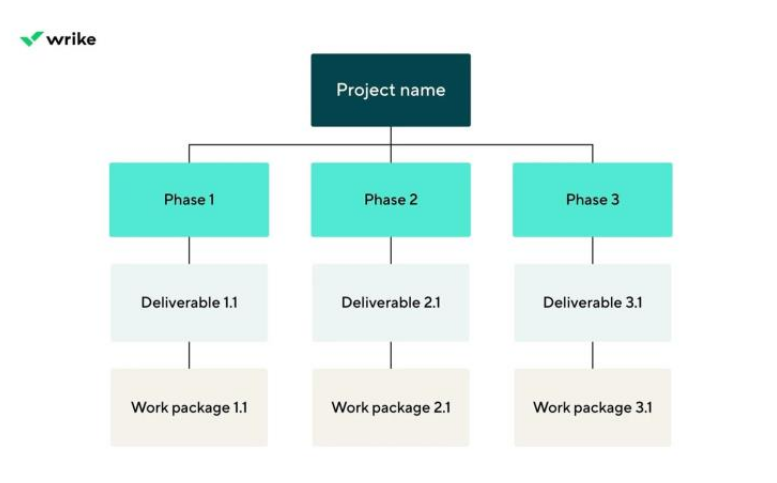
\includegraphics[width=1.0\textwidth]{wrike_2022.png}
  \caption{  Example of project breakdown into work packages. (Source: Wrike,
2022). }
  \label{wrike}
\end{figure*}

\subsection{Resource Requirements}
The following resources are required for the project on over the whole course of
the project:
{\color{red}
\begin{itemize}
\item The numbers and type of personnel: ...
\item Number of computers and software used: ...
\item Office facilities used: ...
\item Training needed: ...
\end{itemize}
}

\subsection{Time Budget and Schedule}
The detailed time budget and schedule is given in document \textcolor{red}{XXX}. The major
activities and tasks, required calendar dates, and their required milestone and
deliverable dates are summarised in Table \ref{tab:time_budget}.

\begin{table}[h]
\centering
\caption{Time budget and schedule for major project activities and tasks.}
\label{tab:time_budget}
\begin{tabular}{|l|c|c|p{2cm}|p{2cm}|}
\hline
\textbf{Activity/Task} & \textbf{Begin} & \textbf{End} & \textbf{Required calendar days} & \textbf{Delivery or milestone date} \\
\hline
 &  &  &  & \\
\hline
 &  &  &  & \\
\hline
 &  &  &  & \\
\hline
 &  &  &  & \\
\hline
\end{tabular}
\end{table}

\section{Additional Components (optional)}

\textcolor{red}{Instructions: Include additional components needed to manage your specific
project. Possibilities include subcontractor management plans, security plans,
training plans, hardware procurement plans, facilities plans, installation plans,
cutover plans, and software maintenance plans.}


\vspace{0.5cm}
\textcolor{red}{If you don’t have any additional components, remove this section, or write: TBD
(To be designed).}

\end{document}
